% !TEX root = comparison.tex
\section{Results and Discussion}~\label{results}

\subsection{Wind Direction and Airport Efficiency}
Figure \ref{fig:time} shows time taken until a decision was made in histograms, facetted by design and colored by correctness of answer. Because of the skewness of the distributions, times were log-transformed. Polar charts take on average more time to answer, but are answered with much lower precision. Figure \ref{fig:conf} shows two barcharts of confidence levels by task, again coloring is used for correctness of answers. Euclidean displays lead to a very bimodal distribution of confidence: participants are either very sure or not sure at all of their answer. Confidence levels in polar charts are distributed much more uniformly.

The perceptual tasks involved in decoding the designs fit into the general framework of the piechart versus barchart discussion. However, we are not dealing with assessing angles, which is known to be a perceptual harder task than assessments of heights or widths in bars, see e.g. \cite{cleveland:1984, robbins:2004, Kosslyn:2006, few:2009}. Instead, the perceptual tasks consists of comparisons along a common axis (in the barcharts) and a common origin (in the polar charts). The difference in designs is therefore based on how well we are able to judge deviations from a horizontal line compared to deviations from a circle. Based on this, the charts with added reference lines provide us with exactly the frame we compare with and should, therefore, be the `better' designs - either in speed or accuracy.

\begin{figure}[hbtp] %  figure placement: here, top, bottom, or page
   \centering
   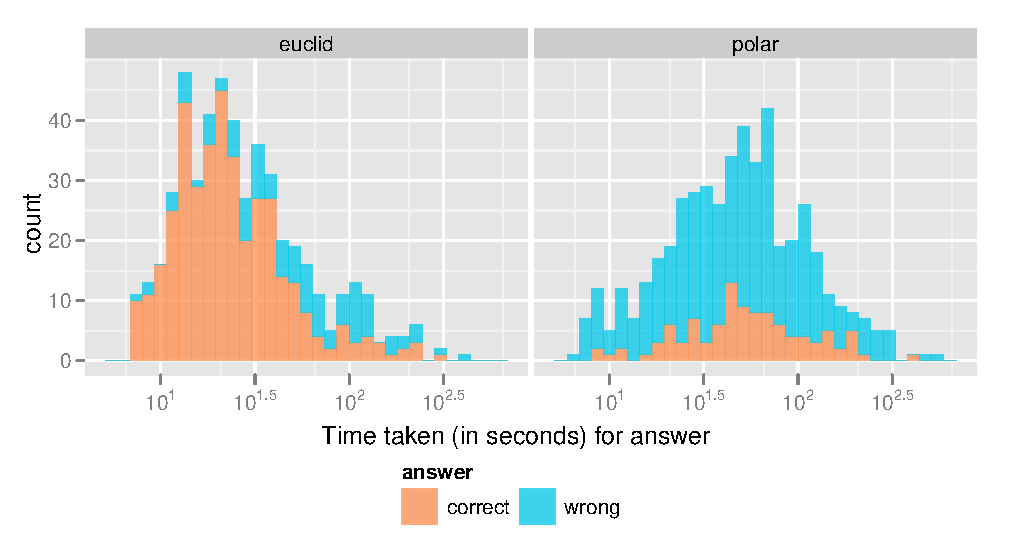
\includegraphics[width=\linewidth]{time-answer} 
   \caption{Histograms of time taken for answering lineups. On average the Euclidean design is answered faster and with higher power (percentage of correct answers). }
   \label{fig:time}
\end{figure}

\begin{figure}[hbtp] %  figure placement: here, top, bottom, or page
   \centering
   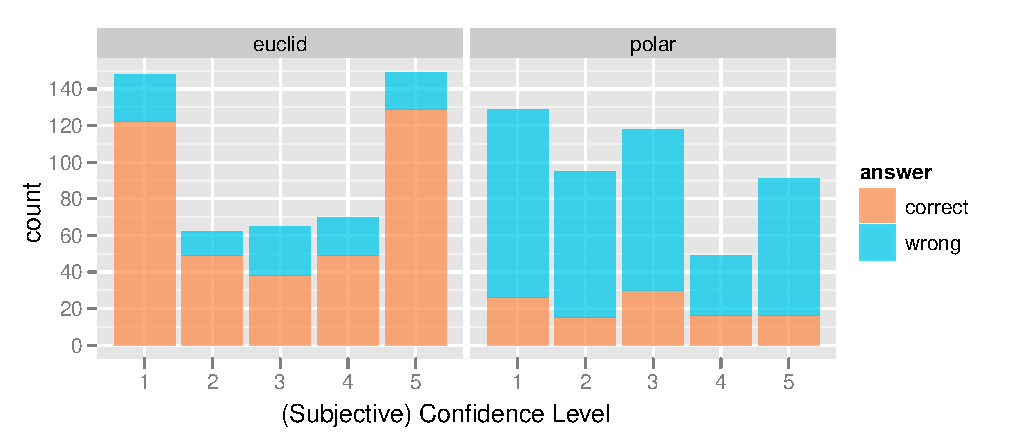
\includegraphics[width=\linewidth]{conf-answer} 
   \caption{Barcharts of (subjective) confidence in answering correctly for each lineup. A strongly bimodal distribution is apparent, while confidence levels for polar charts are more uniform. There are only slight (and non significant) difference between confidence levels and correctness of results.}
   \label{fig:conf}
\end{figure}



%Most generally this experiment can be paralleled to the pie chart versus barchart discussion \cite{***}. 
%The Euclidean coordinate plot is made up of bars where areas are colored proportionally according to percentages. The polar coordinate plot is made up of pie slices which are also colored proportionally according to the data. 
%Viewers of these charts will visually decode the areas of the bars and pie slices and make a judgement based on their decoding. According to  \citet[page=40]{kosslyn:2006}, area is usually perceived as a function of what the actual area is. This function is the area raised to an exponent of approximately 0.8 and then multiplied by a constant. However, when bars are parallel, the relative height of these bars is perceived very accurately. From this information, one could infer that the Euclidean coordinate plot may gain efficiency based on the height of the colored bars. 


For evaluating the results, we are using a generalized linear mixed effects modeling  approach \cite{pinheiro:2000} for all three of our response values, using the {\t R} package {\tt lme4} \cite{bates:2011}. 
For power predictions (cf. table \ref{tbl:correct}) a logistic regression was fitted for the competing designs, including covariates {\it sample size} (2, 4,6, 8, 10, and 24 percent of the data) and {\it shift} in wind direction (offset of 0, 90, 180, and 270 degrees), both as main effects and in two-way interaction effects with design to assess their effect on the power of designs. To adjust for individuals' ability, a random intercept was included in the model.

\begin{figure}[htbp] %  figure placement: here, top, bottom, or page
   \centering

\begin{tabular}{cl}
\phantom{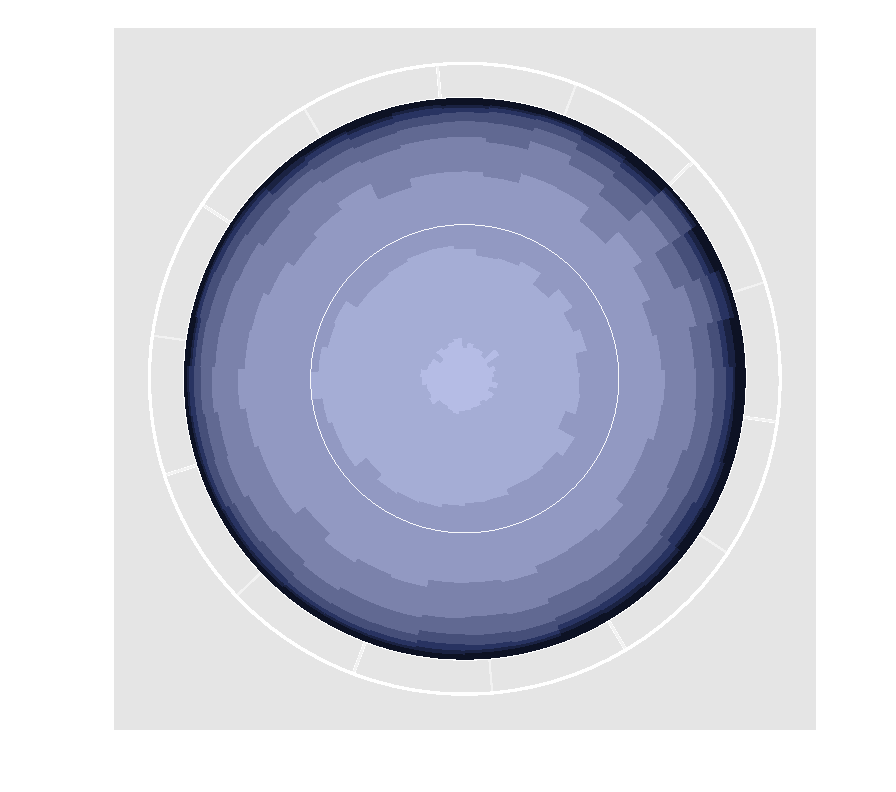
\includegraphics[width=0.03\linewidth]{Polar_Line.pdf}} & \vspace{-0.035in} \multirow{10}{*}{\hspace{-0.25in}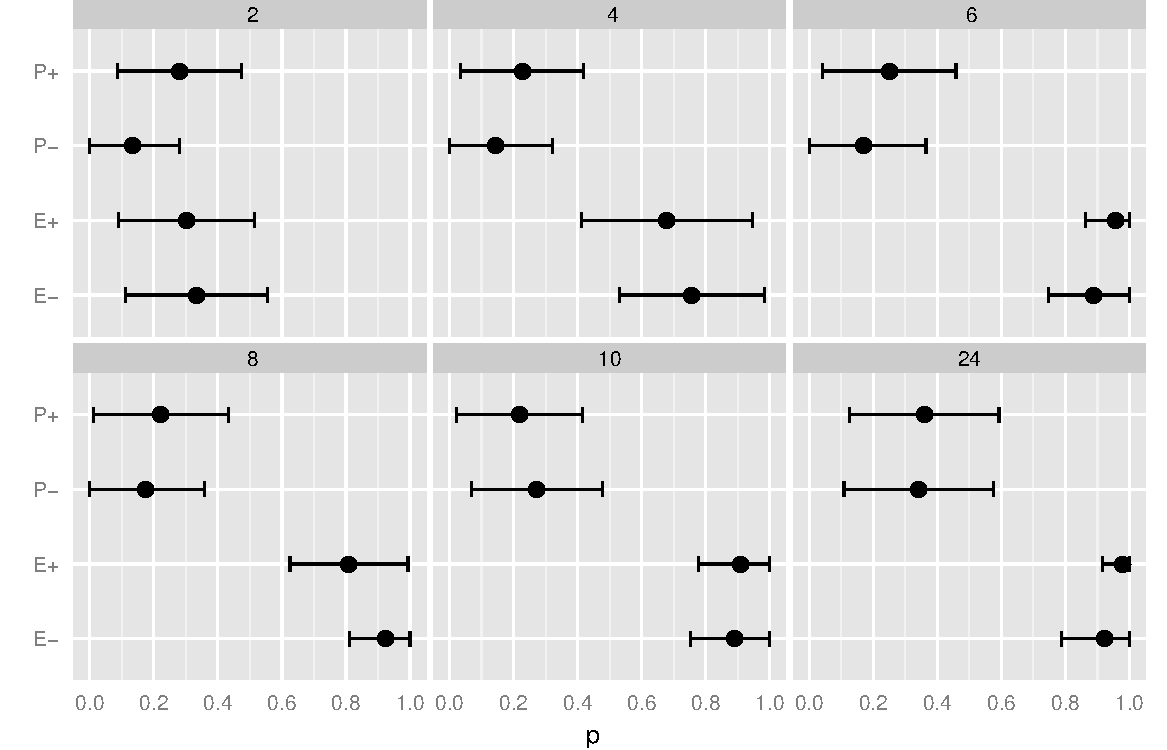
\includegraphics[width=0.9\linewidth]{turk4-designs.pdf}} \\
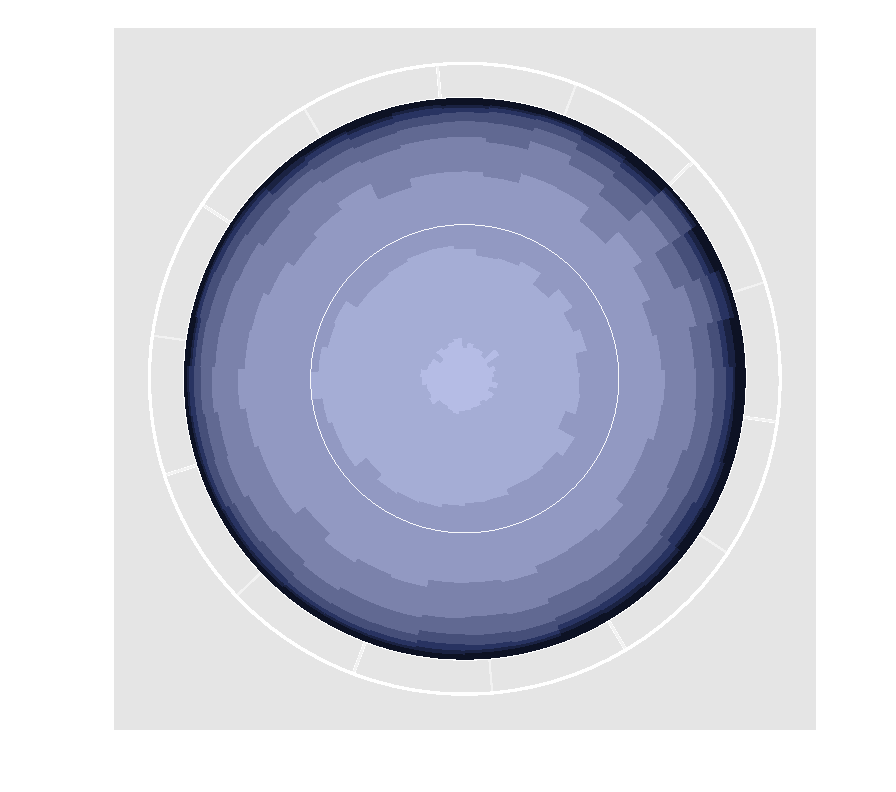
\includegraphics[width=0.05\linewidth]{Polar_Line.pdf} \\
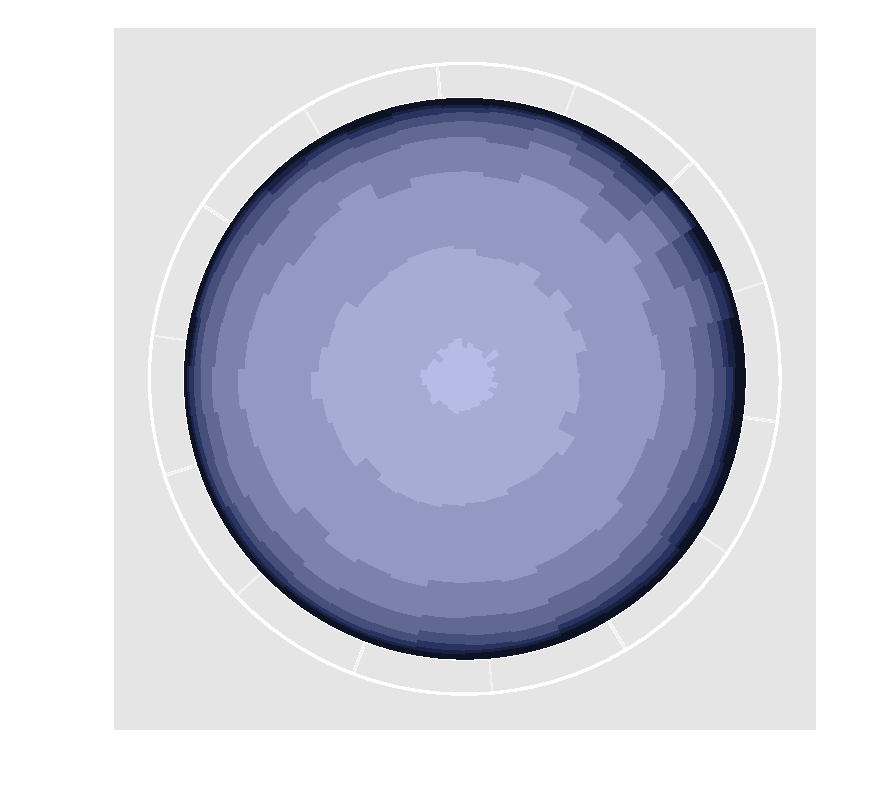
\includegraphics[width=0.05\linewidth]{Polar_NoLine.pdf} \\
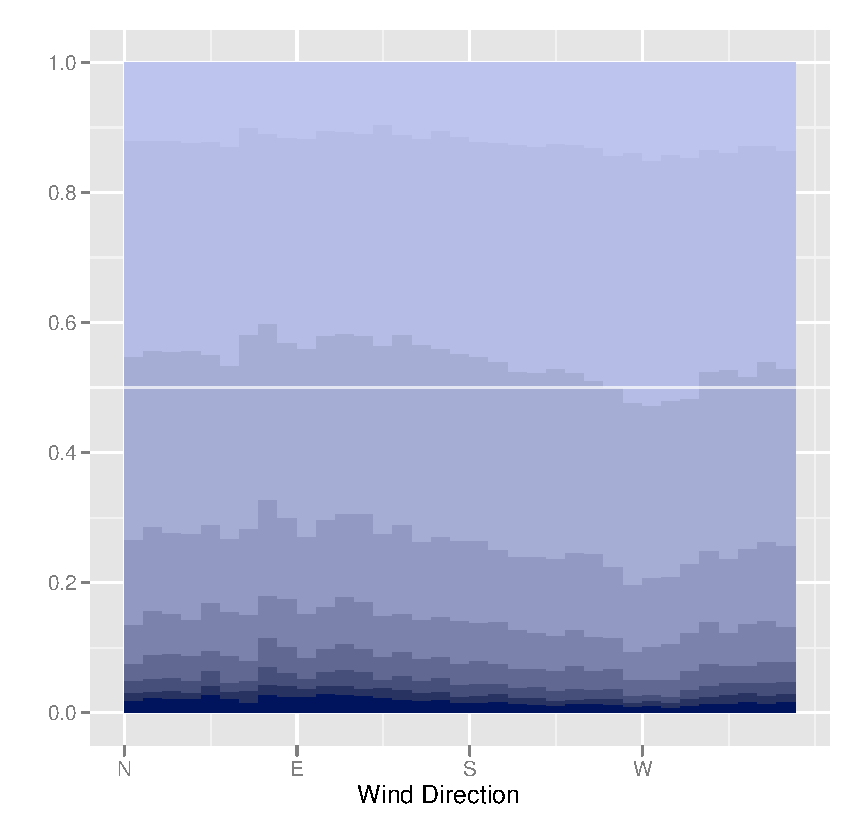
\includegraphics[width=0.043\linewidth]{Euclidian_Line.pdf} \\
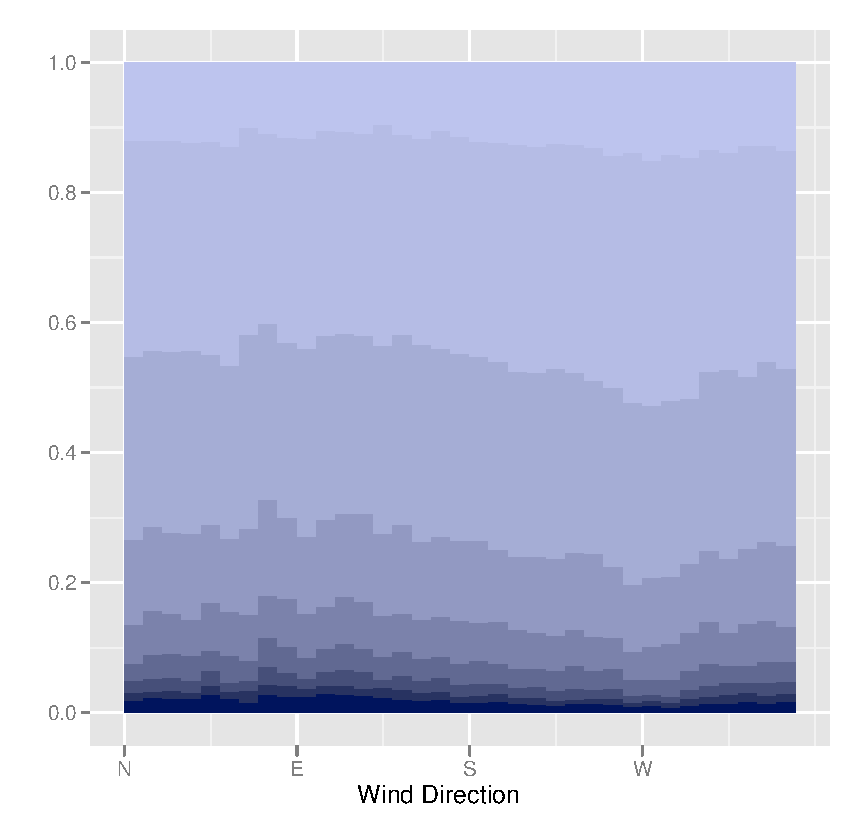
\includegraphics[width=0.043\linewidth]{Euclidian_NoLine.pdf}\\
\phantom{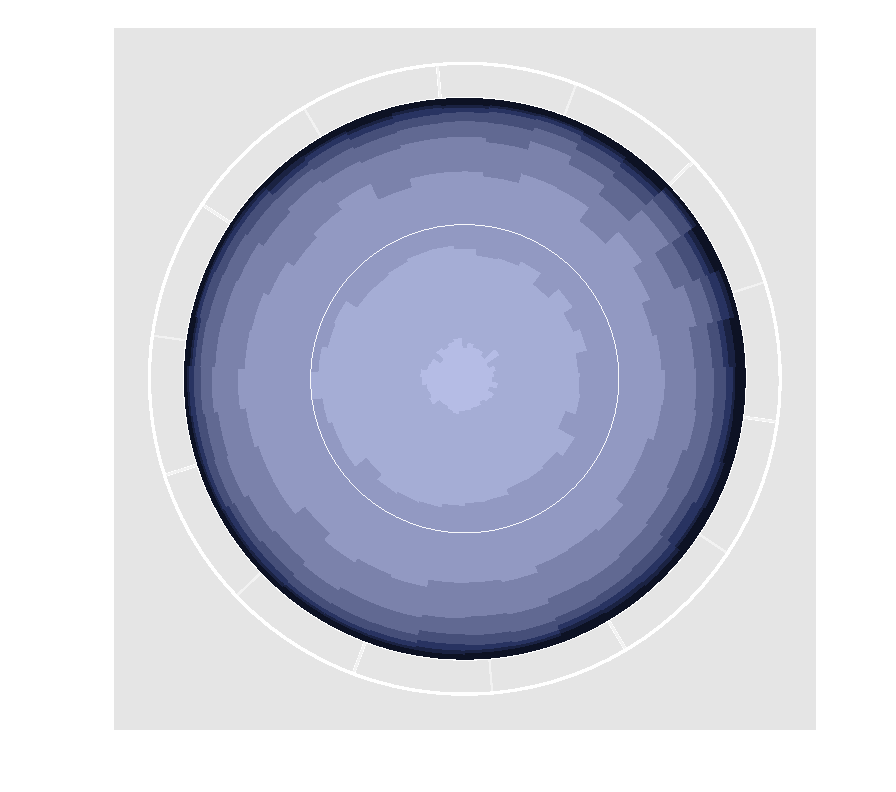
\includegraphics[width=0.015\linewidth]{Polar_Line.pdf}}\\
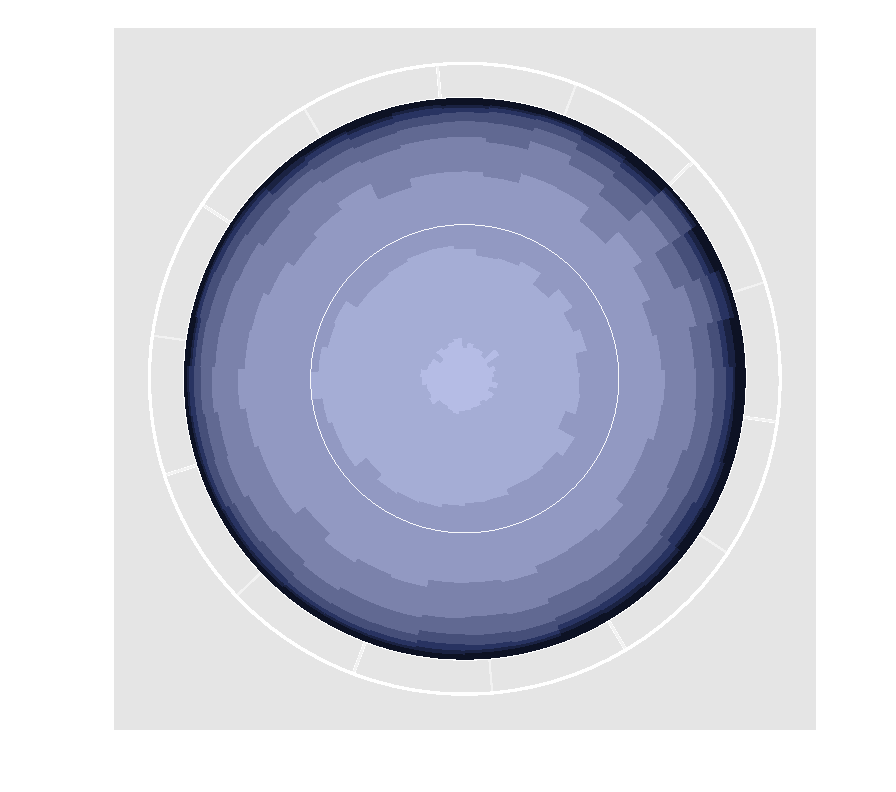
\includegraphics[width=0.05\linewidth]{Polar_Line.pdf} \\
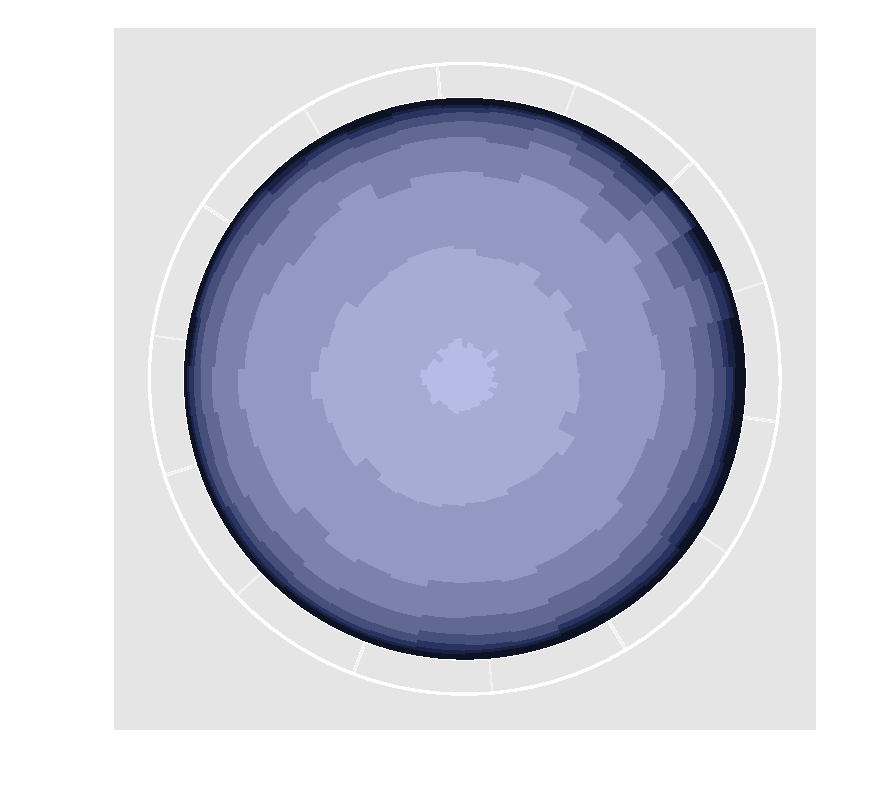
\includegraphics[width=0.05\linewidth]{Polar_NoLine.pdf} \\
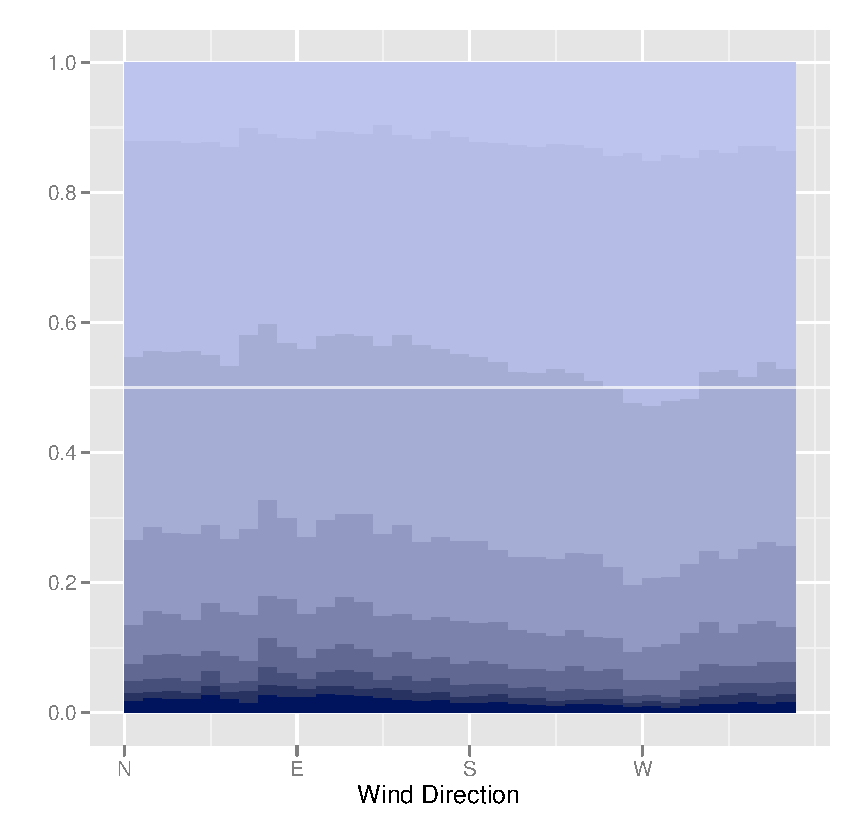
\includegraphics[width=0.043\linewidth]{Euclidian_Line.pdf} \\
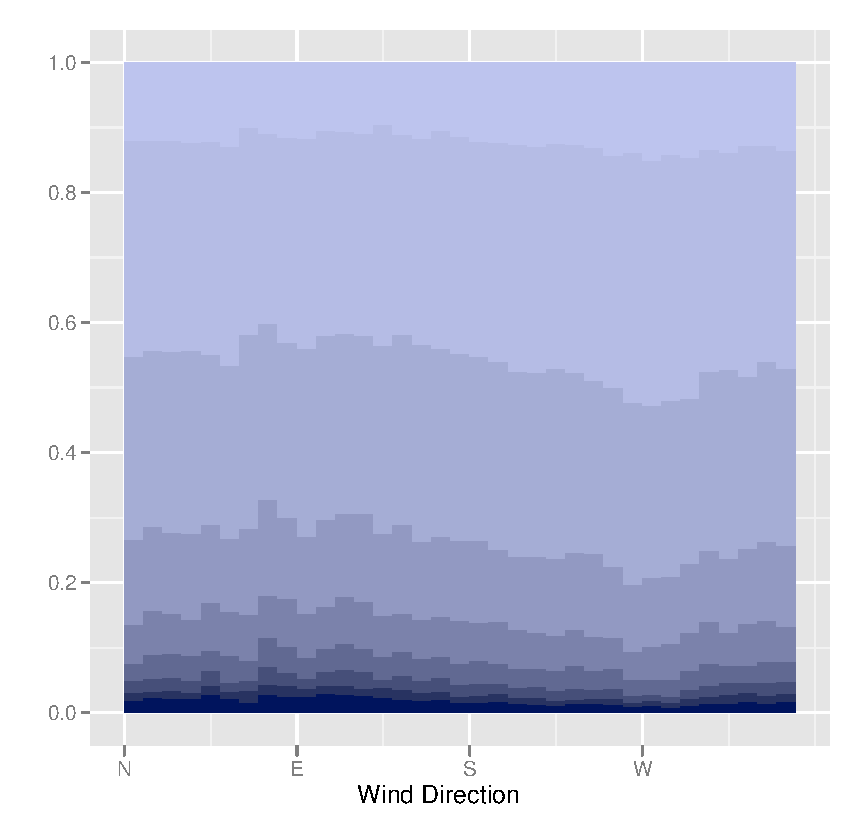
\includegraphics[width=0.043\linewidth]{Euclidian_NoLine.pdf}\\
  \end{tabular} 
  \vspace{0.1in}
   \caption{Power results for two competing designs: polar versus a Euclidean, with and without a reference line. Error bars indicate 95\% confidence intervals. Plots are facetted by percentage of data used. }
   \label{fig:treatment}
\end{figure}


Overall, the results show huge differences in the power of designs between polar charts and Euclidean: Euclidean designs are significantly more powerful than polar charts, particularly so with small sample sizes. 76.92\% of the Euclidean lineups shown resulted in the a correct identification of the real data while only 20.31\% of the polar charts were correct.
 The reference line has surprisingly little influence, but it helps more for  polar charts than for Euclidean charts,
An increase in sample size has positive impact on power (see figure \ref{fig:treatment} for an overview). Polar charts need a much bigger sample size to see an increase in power -- only at about 24\% of the original data do we see about the same power as for Euclidean charts of a sample size of 2\%.
The  changes in offset are significant -- interestingly, borderline behavior (90 and 270 degrees) does not show a difference between polar and Euclidean charts, whereas an inversion of the wave pattern (first up, then down), does show a difference. The power of Euclidean lineups suffers significantly  from this inversion whereas power of polar charts is unaffected. This is an unexpected finding, but is consistent throughout different lineups in the data. Figure \ref{fig:power} summarizes the results from the model: power predictions ($y$ axis) are shown by sample size ($x$ axis). The thick lines show average power by design for different shifts in wind direction. The thin lines represent power for individuals. What can be seen is the different impact of the offset by design: while  an offset of 270 degrees (the 'mountain' pattern) has the highest power in Euclidean charts, it comes out worst in polar charts.

\begin{figure}[htbp] %  figure placement: here, top, bottom, or page
   \centering
   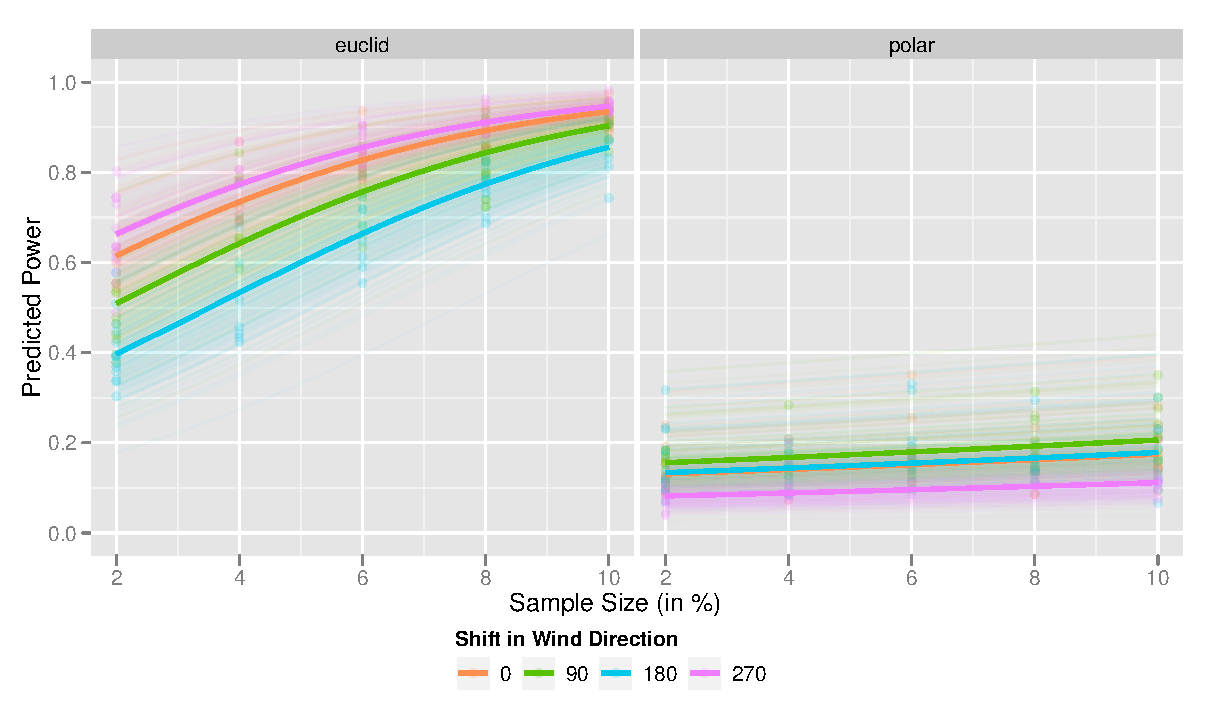
\includegraphics[width=\linewidth]{predict-power} 
   \caption{Predicted Power of designs.  The thin lines and the points on $y$ axis show  variability due to individuals' abilities. The saturated lines show average predicted power for each of the designs.}
   \label{fig:power}
\end{figure}

Time taken to answer was log transformed before the modeling process to de-emphasize the impact of very large values (up to 500 sec). The findings are consistent with correctness - time taken shows big differences between polar and Euclidean charts. The average of the amount of time spent on a Euclidean lineup is 3.53 minutes while it was 4.07 minutes for a polar lineup.
The reference lines seem to increase the evaluation time, but not significantly. An increase in sample size decreases evaluation time, The inversion of the wave pattern at 180 degrees leads to a significant increase in time for Euclidean charts, but not for polar charts (at least not significantly). 


 Confidence levels are measured on a five point scale --- they are subjective assessments by the participant `how certain are you'. We model confidence using the same model structure as before, i.e. using sample size and offset as covariates and including up to two-way interactions,
While there is a difference between the designs - participants reported higher confidence in dealing with the Euclidean lineups -- this is only  a trend (i.e. not significant at 5\% but below 10\%). The only significant effect on reported confidence level is the use of reference lines in polar coordinates: participants report an increase in confidence (0.31 $\pm$ 0.13, $p$ value = 0.01) when using the reference line. This, however, does not translate to a significant increase in accuracy of results, as we have seen before.

 Euclidean coordinates resulted in a significantly more accurate identification of the real data set in significantly shorter time.

\begin{table}[ht]
\begin{center}
\resizebox{\linewidth}{!} {
%\rowcolors{2}{white}{lightgray}
\begin{tabular}{rrrrrrl}
  \hline
& & Estimate & Error & $z$-value & $p$-value &\\ 
  \hline
\bf design & euclid & -0.08 & 0.39 & -0.21 & 0.84 &\\ 
&polar & -1.98 & 0.32 & -6.13 & 0.00 & ***\\ [3pt]
\multicolumn{2}{l}{\bf main effects} &&&&&\\
& reference line  & -0.14 & 0.26 & -0.53 & 0.59 & \\ [1pt]
&  sample size & 0.27 & 0.04 & 6.31 & 0.00 & ***\\[1pt]
 &offset:  90 degrees& -0.43 & 0.37 & -1.18 & 0.24 &\\ 
  & 180 degrees& -0.89 & 0.35 & -2.51 & 0.01 & **\\ 
  & 270 degrees& 0.21 & 0.38 & 0.55 & 0.58 &\\ [3pt]
\multicolumn{2}{l}{\bf interactions} &&&&&\\
&  polar:line & 0.51 & 0.35 & 1.44 & 0.15 &\\ [1pt]
&    polar:sample size & -0.23 & 0.05 & -5.02 & 0.00 & ***\\[1pt]
&    polar:offset 90 & 0.64 & 0.49 & 1.30 & 0.20 \\ 
&  polar:offset 180 & 0.91 & 0.47 & 1.92 & 0.05 & .\\ 
&    polar:offset 270 & -0.73 & 0.54 & -1.35 & 0.18 &\\
   \hline
\\[-5pt]
   \multicolumn{5}{l}{Signif. codes:  0 `***' 0.001 `**' 0.01 `*' 0.05 `.' 0.1}
\end{tabular}
}
\end{center}
\caption{\label{tbl:correct} Output of a generalized linear mixed effects model for power of lineups (i.e. probability of identifying the data plot) for comparing designs. Included are two-way interactions with sample size and shifts in wind direction (offset). Euclidean designs without a reference line at offset 0 are used as 
 Results are based on  976 lineup evaluations by 115 participants. }
\end{table}


\begin{table}[ht]
\begin{center}
\resizebox{\linewidth}{!} {
%\rowcolors{2}{white}{lightgray}
\begin{tabular}{lrrrrrl}
  \hline
& & Estimate & Error & $t$-value & \multicolumn{2}{l}{approx $p$-value} \\   \hline
\bf design & Intercept & 3.58 & 0.09 & 41.34 & 0.00 & ***\\ 
&  polar & 0.22 & 0.10 & 2.17 & 0.03 & * \\ [2pt]
\multicolumn{2}{l}{\bf covariates}\\
&reference line & 0.08 & 0.06 & 1.50 & 0.13 \\ [1pt]
 & sample size & -0.03 & 0.00 & -8.73 & 0.00 & ***\\ [1pt]
&  offset: 90 & -0.06 & 0.08 & -0.72 & 0.47 \\ 
& 180 & 0.16 & 0.08 & 2.07 & 0.04 & *\\ 
&  270 & -0.04 & 0.07 & -0.54 & 0.59 \\ [2pt]
\multicolumn{2}{l}{\bf interactions}\\
&  polar:line & -0.03 & 0.08 & -0.40 & 0.69 \\ [1pt]
&    polar:sample size & 0.03 & 0.01 & 6.25 & 0.00 & ***\\ [1pt]
&    polar:offset 90 & 0.14 & 0.11 & 1.23 & 0.22 \\ 
&    polar:offset 180 & -0.17 & 0.11 & -1.55 & 0.12 \\ 
&    polar:offset 270 & 0.17 & 0.11 & 1.50 & 0.13 \\ 
   \hline
\\[-5pt]
   \multicolumn{5}{l}{Signif. codes:  0 `***' 0.001 `**' 0.01 `*' 0.05 `.' 0.1}
\end{tabular}}
\end{center}
\caption{\label{tbl:time} Model output for linear mixed effects model of (log) time taken, barchart design is baseline. }
\end{table}


%Euclidean coordinates performed better when speaking of efficiency in terms of accuracy and speed. 76.92\% of the Euclidean charts shown resulted in the a correct identification of the real data while only 20.31\% of the polar charts did the same. A t-test comparing means for charts with polar coordinates versus charts with Euclidean coordinates resulted in a t statistic of 15.2013 with a p-value of 2.2e-16. Similarly, a t-test comparing means of time spent on charts with Euclidean coordinates versus charts with polar coordinates resulted in a p-value of 1.014e-11. The average of the log of time spent on each individual chart for charts with Euclidean coordinates is 3.53 minutes while it was 4.07 minutes for charts with polar coordinates. Euclidean coordinates resulted in a significantly more accurate identification of the real data set in significantly shorter time. 

%\begin{figure}[htbp] %  figure placement: here, top, bottom, or page
%   \centering
%   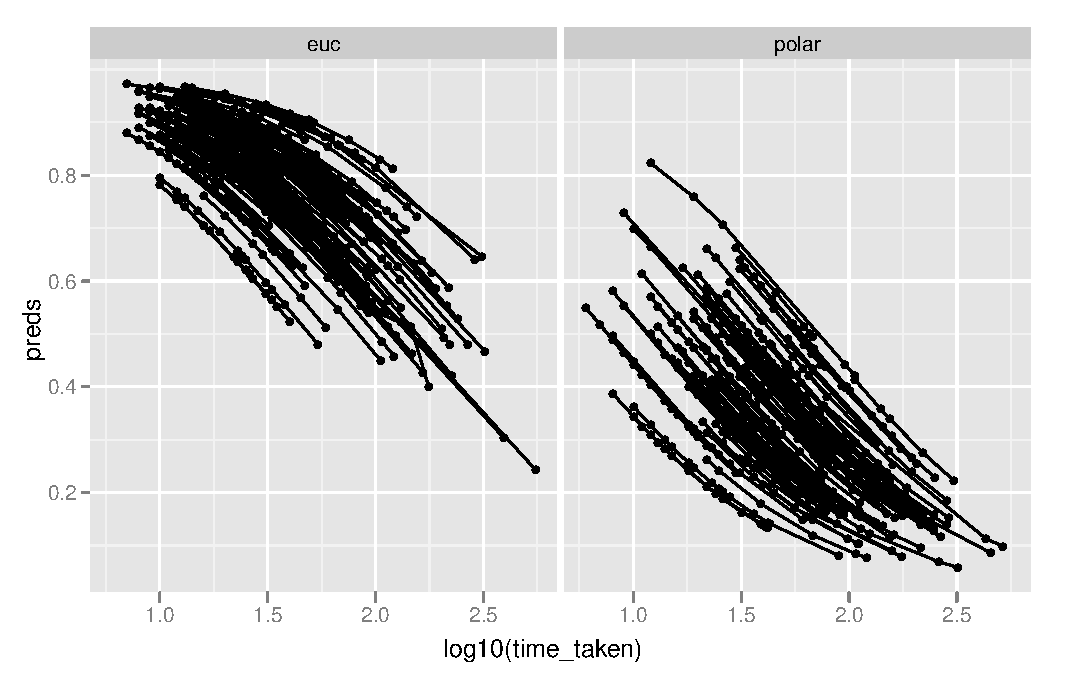
\includegraphics[width=3in]{turk4_time_perc_preds.pdf}  
%   \caption{Values predicted from XXXX how to say itXXXX of accuracy for log of time taken and test parameter.}
%   \label{accuracy_preds}
%\end{figure}
%
%Figure \ref{accuracy_preds} shows predicted accuracy levels. These predicted values were obtained by using R package lme4 and a mixed effect model explaining correct responses by type of chart and the log of time spent while accounting for different levels of accuracy for each individual who participated in the experiment. The predicted values show that there is an overall higher accuracy level for Euclidean coordinates when compared to polar coordinates. For both chart types, as the time spent increases, the predicted accuracy decreases. 
%
%\begin{figure}[htbp] %  figure placement: here, top, bottom, or page
%   \centering
%   %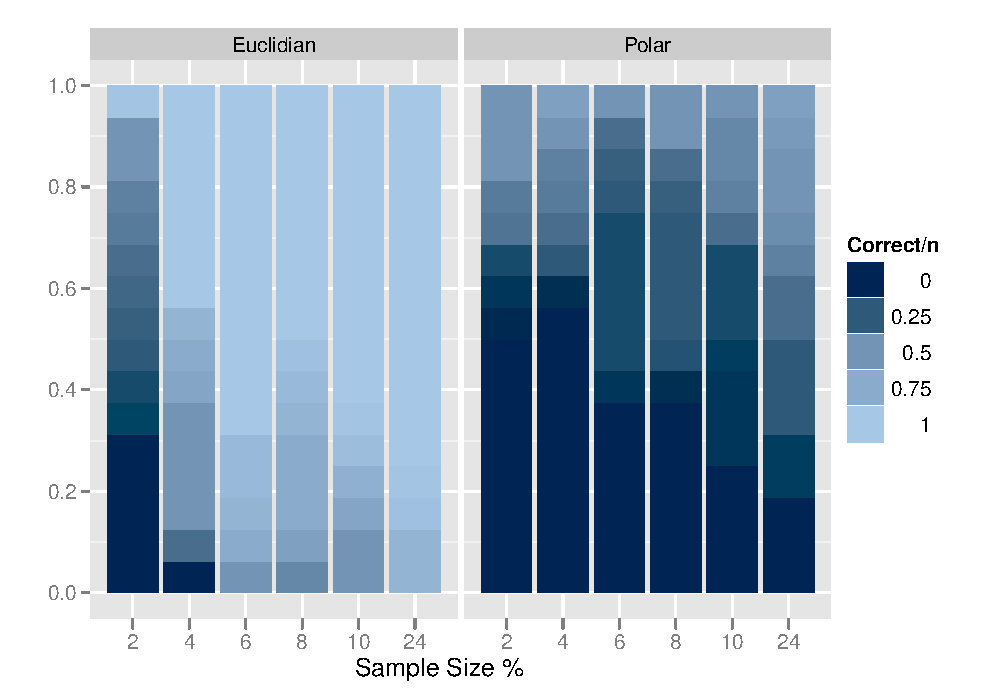
\includegraphics[width=3in]{turk4_samplesize_correctn.pdf}  
%   \caption{For each sample size for polar and Euclidean coordinates, the bars are colored according to the number of correct responses. Darker colors indicate lower accuracy levels while lighter colors indicate higher accuracy levels. }
%   \label{samp_size_acc}
%\end{figure}

%Ideally, efficient detection of data characteristics will be possible at small sample sizes. The difficulty of the charts is largely determined by the sample size taken from the original data set. Samples of 24 \% generally result in higher accuracy as the extra information facilitates detection of a relationship. Figure \ref{accuracy_preds} shows the relationship between the number of correct responses relative to the total number of responses and how this relationship differs between Euclidean and polar coordinates. The bars in the Euclidean plot are overall a lighter color than they are in the polar plot. This indicates a higher level of accuracy at all sample sizes. For Euclidean coordinates, we can see a stair step pattern in the accuracy levels as sample size increases. Lower levels of accuracy, indicated by darker colors, become consistently less prevalent as sample size increases. The relationship between sample size and accuracy level is not as simple for polar coordinates. Sample sizes of 2\% and 4\% have very similar accuracy levels. After 6\% the stair step pattern becomes visible and similar to that of Euclidean coordinates. Sample size seems to have less of an effect on accuracy for polar coordinates than it does for Euclidean coordinates. Predicted values of the proportion of correct responses when explained by sample size, the type of chart, and the interaction between these two factors, show that there is a significant difference between the relationship between sample size and correct responses for polar and Euclidean coordinates. Indeed, the proportion of correct responses increases more rapidly as sample size increases for Euclidean coordinates than it does for polar coordinates. 
%
%The effect of a reference line on accuracy and time was not statistically significant for both types of charts. When looking at plots of the data, however, the time spent on the charts seems to be higher when there is a reference line.This is true for both Euclidean and polar charts. Also visible in the data is a slight increase in accuracy with the presence of a reference line. These characteristics can be seen in figure\ref{reflines}.  
%
%\begin{figure}[htbp] %  figure placement: here, top, bottom, or page
%   \centering
%   %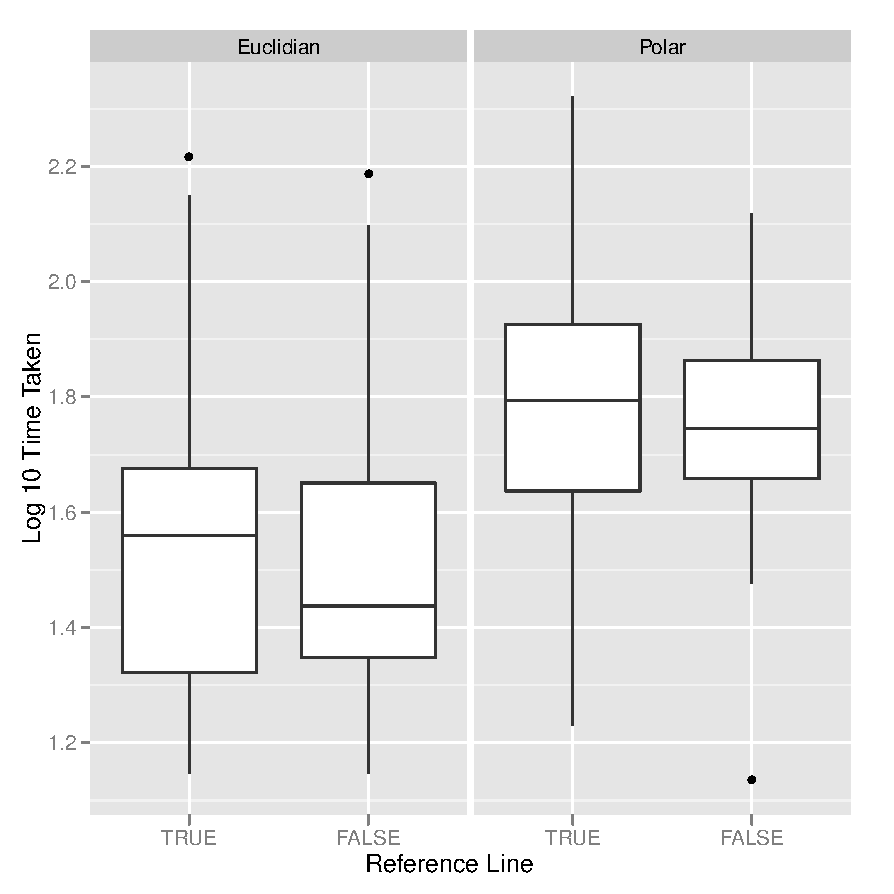
\includegraphics[width=1.5in]{turk4_refilne_time.pdf}  
%   %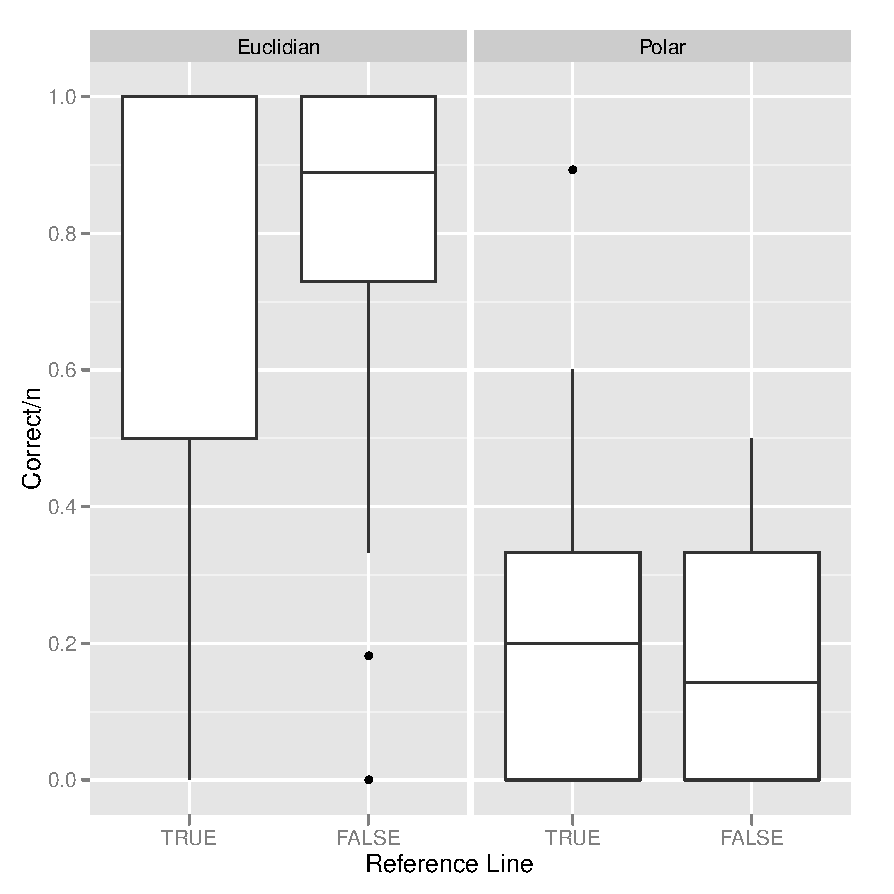
\includegraphics[width=1.5in]{turk4_refline_correctn.pdf}  
%   \caption{The relationship between reference line and time spent (left) and the relationship between reference line and accuracy (right). Although not statistically significant, some patterns are visible.}
%   \label{reflines}
%\end{figure}







